\documentclass[a4paper,10pt]{article}
\usepackage{ucs}
\usepackage[utf8x]{inputenc}
\usepackage[german]{babel}
\usepackage{fontenc}
\usepackage{graphicx}
\usepackage{fullpage}
\usepackage{hyperref}

\author{Sebastian Kumminger\\
	Fabian Schneider\\
	Tobias Himmer}

\title{Pflichtenheft\\
	Elektronische Betreuungsplanung und Tagesdokumentation}

\date{22.11.2011}

\begin{document}

\maketitle

\tableofcontents
\newpage

\section{Produktbeschreibung}
\subsection{Übersicht}
Das Ziel ist es, eine Applikation zu entwickeln, die es Einrichtungen der Behinderten- und Altenhilfe ermöglicht,
die langfristige Betreuungsplanung mit der Tagesdokumentation zu verknüpfen. Es sollen Ereignisse aus dem Tagesgeschehen,
die in der Tagesdokumentation der Wohngruppe / des Pflegeheims erfasst werden,
der Betreuungsplanung des bertoffenen Bewohners zugeordnet werden können.
Damit soll doppelter Dokumentationsaufwand verhindert werden.
\subsection{Anwendungsbereiche}
Die Software soll in stationären und ambulanten Einrichtungen der Behindertenhilfe in Baden Württemberg eingesetzt werden. 
Diese Einschränkung ergibt sich aus der Implementierung der Betreuungsplanung. Diese Version orientiert sich an dem aktuell in Baden Württemberg geltenden 
Standard, dem Metzler-Verfahren. 
\subsection{Zielgruppe}
Die Software soll vorwiegend von pädagogischen Fachkräften benutzt werden. Entsprechend den individuellen Arbeitsabläufen in den 
Einrichtungen der Behindertenhilfe ist auch eine Bedienung durch Personal auf Leitungsebene (Heimleitung) denkbar.
\subsection{Betriebsbedingungen}
Um eine höhere Datensicherheit zu gewährleisten, soll die Anwendung auf einem
zentralen Server ausgeführt werden und von einem, oder mehreren externen Clients gleichzeitig bedienbar sein.
Der Zugriff der Clients soll über eine Remotedesktopumgebung erfolgen.
Dies unterbindet den direkten Zugriff auf die Datenbank und versucht damit den gesetzlichen Verpflichtungen (Siehe Kapitel \pageref{subsec:dasi}) nachzukommen.

\section{Funktionsumfang}
\subsection{Kernfunktionen}
\subsubsection{Rechteverwaltung}
\begin{itemize}
	\item Mitarbeiter und Bewohner werden einer Wohngruppe zugeordnet.
	\item Jeder Mitarbeiter darf nur auf die Bewohner seiner Wohngruppe zugreifen.
\end{itemize}
\subsubsection{Bewohnerverwaltung}
\begin{itemize}
	\item Personenbezogene Informationen
	\item Planung von Projekten
	\begin{itemize}
		\item Verknüpfung zur Betreuungsplanung
	\end{itemize}
	\item Protokollfunktion
	\begin{itemize}
		\item Verknüpfung zur Betreuungsplanung
	\end{itemize}
	\item  Betreuungsplanung
	\begin{itemize}
		\item Betreuungsplanung nach einem aktuellen Standard der Alten- oder Behindertenhilfe
		\item Übernahme von Ereignissen aus der Tagesdokumentation in die Kategorien der Betreuungsplanung
	\end{itemize}
\end{itemize}
\subsubsection{Tagesdokumentation}
\begin{itemize}
	\item Gruppenbuch
	\begin{itemize}
		\item Gruppenbezogene Ereignisse werden mit Uhrzeit und Mitarbeiternamen erfasst
		\item Klientenbezogene Ereignisse können in die Betreuungsplanung des entsprechenden Klienten übertragen werden.
		\item Such- und Listenfunktion für die klientenbezogenen Ereignisse
		\item Meldeliste für alle Bewohner
		\begin{itemize}
			\item Urlaub, Krankheit, Abwesenheit mit Grund
			\item Export der Meldeliste in einem gängigen Format (z.B. CSV, XML)
		\end{itemize}
	\end{itemize}
\end{itemize}
\subsubsection{Multilinguale Oberfläche}
Unterstützte Sprachen
\begin{itemize}
	\item Deutsch
	\item Englisch
%	\item Esperanto
%	\item Klingonisch
\end{itemize}
\subsection{Zusatzfunktionen}
\subsubsection{Bewohnerverwaltung}
\begin{itemize}
	\item Adressverwaltung
	\item Planung von Aufgaben
	\item Generierung bestimmter Dokumente aus den Daten der Datenbank
	\begin{itemize}
		\item Z.B. Heimvertrag
	\end{itemize}
\end{itemize}
\subsubsection{Tagesdokumentation}
\begin{itemize}
	\item Tagesplan / Wochenplan
	\begin{itemize}
		\item Alle Aktivitäten / Aufgaben an einem bestimmten Tag / über einen bestimmten Zeitraum.
		\item Termine können als ics Termin an einen E-Mailempfänger verschickt werden
	\end{itemize}
\end{itemize}
\subsubsection{Sonstiges}
\begin{itemize}
	\item Der Zugriff von Clientrechnern kann auch über einen gesonderten \label{Serverdaemon} Serverdaemon erfolgen,
	der den Datenfluss zwischen Client und Datenbank kontrolliert.
\end{itemize}


\section{Technische Produktumgebung}
\subsection{Softwareanforderungen}
\subsubsection{Server}
\begin{itemize}
	\item Betriebssystem: aktuelle GNU/Linux Distribution;
	\item MySql Server
	\item Ein beliebiger Remote-Desktop Dienst.
	\item Bibliotheken: Qt4, ODB;
\end{itemize}
\subsubsection{Client}
\begin{itemize}
	\item Beliebiges Betriebssystem mit Remote-Desktop;
\end{itemize}
\subsection{Hardwareanforderungen}
\subsubsection{Server}
\begin{itemize}
	\item Arbeitsspeicher: 1 GB
	\item NIC: 100 Mbit/s
\end{itemize}
\subsubsection{Client}
\begin{itemize}
	\item NIC: 100 Mbit/s
	\item Eingabegeräte: Maus + Tastatur
	\item Monitor mit mindestens 800x600 Pixel Auflösung
\end{itemize}
\subsection{Anforderungen an die Organisation (Orgware)}
Soll aus dem Internet auf den Server zugegriffen werden, ist die Internetanbindung entsprechend der verwendeten Remote-Desktop Konfiguration / Benutzerzahl zu dimensionieren.
\subsection{Produktschnittstellen}
\subsubsection{Object-Relational-Mapper}
Um die Entwicklungsdauer zu verkürzen und die Wartbarkeit der Persistenzschicht zu erhöhen, wird ein Object Relational Mapper (ORM) eingesetzt. 
Dieser hilft die relationale Tabellenstruktur der Datenbank auf Objekte der Programmiersprache abzubilden.
Das verwendete Qt4-Toolkit enthält zwar eine plattformunabhängige Schnittstelle für Datenbanken (QtSql), jedoch hat diese keine ORM Funktion.
Folgende ORM-Systeme wurden in Betracht gezogen \newline\url{http://en.wikipedia.org/wiki/List_of_object-relational_mapping_software}:
\begin{itemize}
	\item LiteSQL - Datenbankschema wird mit XML Dateien beschrieben
	\item ODB - Datenbankschema wird aus den C++ Klassen generiert
	\item QxOrm - Benutzt QtSql; Unter Umständen müssen direkte Aufrufe von QtSql erfolgen
	("QxOrm cannot resolve all problems with sql and databases, so it is sometimes necessary to use QtSql engine of Qt library to write your own sql query or stored procedure." \url{http://www.qxorm.com/qxorm_en/tutorial.html})
\end{itemize}
Alle Systeme bieten eine Qt Integration, die die Schnittstelle zwischen GUI und Persistenzschicht vereinfachen.
Ebenso unterstützen alle Systeme mehrere Datenbankbackends.
Letztendlich fiel die Entscheidung auf ODB, da diese Bibliothek (unter anderem durch Caching) die beste Performance verspricht.
Ausserdem lassen sich Klassen mit geringem Aufwandt persistent machen.
\subsubsection{Datenbank}
Als Datenbank wird MySQL eingesetzt. Diese ist für nicht-kommerzielle Zwecke (im Sinne der GPL) frei erhältlich und sehr weit verbreitet. 
Ein Wechsel auf eine andere Datenbank (zum Beispiel PostgreSQL) sollte dank ODB ohne größere Probleme möglich sein.
%TODO: evtl noch QT

\section{Anforderungen an die Entwicklungsumgebung}
\subsection{Softwareanforderungen}
\begin{itemize}
	\item Datenbank: MySql-Client Entwicklungsbibliothek;
	\item GUI: Qt-SDK; 
	\item ORM: ODB-SDK;
	\item Buildtools: CMake, GCC;
\end{itemize}
\section{Grafische Benutzeroberfläche}
\subsection{Grundlegende Anforderungen}
Um die Usability und das Look-and-Feel einer Desktopanwendung zu gewährleisten, wird ein GUI Toolkit verwendet.
Hierfür soll Qt4 zum Einsatz kommen. Qt ist zum einen portabel auf verschiedene Plattformen 
und bietet neben den grafischen Bedienelementen eine breite Auswahl an Schnittstellen zu Systemfunktionen.
\subsection{Anforderungen an die Verknüpfung der Betreuungsplanung}
Eine der Hauptfunktionen soll das Zuordnen von Tagesereignissen zu den Zielen der Betreuungsplanung sein. Diese Funktion soll über 
kurze und intuitive Wege erreichbar sein. Die Usability dieser Funktion steht im Vordergrund.
\subsection{Mockup}
Abbildungen \ref{Info} und \ref{Protokoll} auf Seite \pageref{Info} / \pageref{Protokoll}  zeigen eine mögliche Darstellung der graphischen Benutzeroberfläche. 
Die GUI besteht im Wesentlichen aus drei Teilen. Auf der linken Seite befindet sich das Menü. Die einzelnen Menüpunkte sind dabei in einer Baumstruktur angeordnet. 
Zusätzlich sind die Menüpunkte für Funktionen die die Wohngruppe betreffen von den Funktionen die sich auf Bewohner beziehen getrennt. 
Durch Registerkarten kann zwischen diesen Menüs gewechselt werden. Im oberen Teil der GUI befindet sich ein Panel, das Informationen über die aktuell selektierte Wohngruppe bzw. den aktuellen Bewohner anzeigt. 
In der Mitte befindet sich die Hauptansicht. Dort wird der aktuelle Menüpunkt dargestellt. Seitenmenü und Informationspanel werden als Dockwidget erstellt und können 
somit von dem User aus dem Hauptfenster gelöst werden. Auch die Platzierung an anderer Stelle ist möglich. So könnte das Menü auch auf der rechten Seite angebracht werden.
\newline
Abbildung \ref{Info} zeigt die Darstellung der personenbezogenen Daten. Im Menü ist zu erkennen, dass der Menüpunkt \emph{Person} noch weitere Unterpunkte hat. 
Je nach eingestelltem Look and Feel werden die Unterpunkte auch eingerückt dargestellt.

\section{Qualitätssicherung}
\subsection{Usability}
Die Usability der grafischen Bedienoberfläche soll in zwei Stufen getestet werden.
\begin{itemize}
	\item Es wird ein horizontaler Prototyp erstellt,  um die grafischen Bedienelemente auf verschiedene Anwendungsfälle vorab zu testen. 
	\item Für die funktionsfähige Anwendung soll der Alltagsgebrauch simuliert werden, um nicht erkannte Anwendungsfälle oder Fehlverhalten zu entdecken.
\end{itemize}
Die Probanden der Usability-Tests sollen aus der Zielgruppe sein, um besondere Bedürfnisse erkennen zu können.    
\subsection{Codequalität}
Die Codequalität soll durch Unit Tests gewährleistet werden.
Die Unittests werden mit Hilfe der QtTest Bibliothek und dem CUnit Framework entwickelt.
Zusätzlich wird, um Programmierfehler frühzeitig aufzuspüren, ein Speicherdebugger (valgrind) eingesetzt.

\section{Nichtfunktionale Anforderungen} \label{sec:anf}
%\subsection{Barrierefreiheit}
\subsection{Datensicherheit} \label{subsec:dasi}
Die personenbezogenen Daten von Bewohnern einer stationären Einrichtung der Behindertenhilfe sind im besonderen Maße zu schützen. Bei der Erhebung und Speicherung ist darauf zu achten, dass dies im Rahmen der Normen des Sozialgesetzbuches (§35 SGB I und §§ 67 SGB 10 ff) geschieht.
\subsection{Lizenzen}
Die Software wird unter GPLv3 lizensiert und veröffentlicht.
%\section{Termine}

\begin{figure}
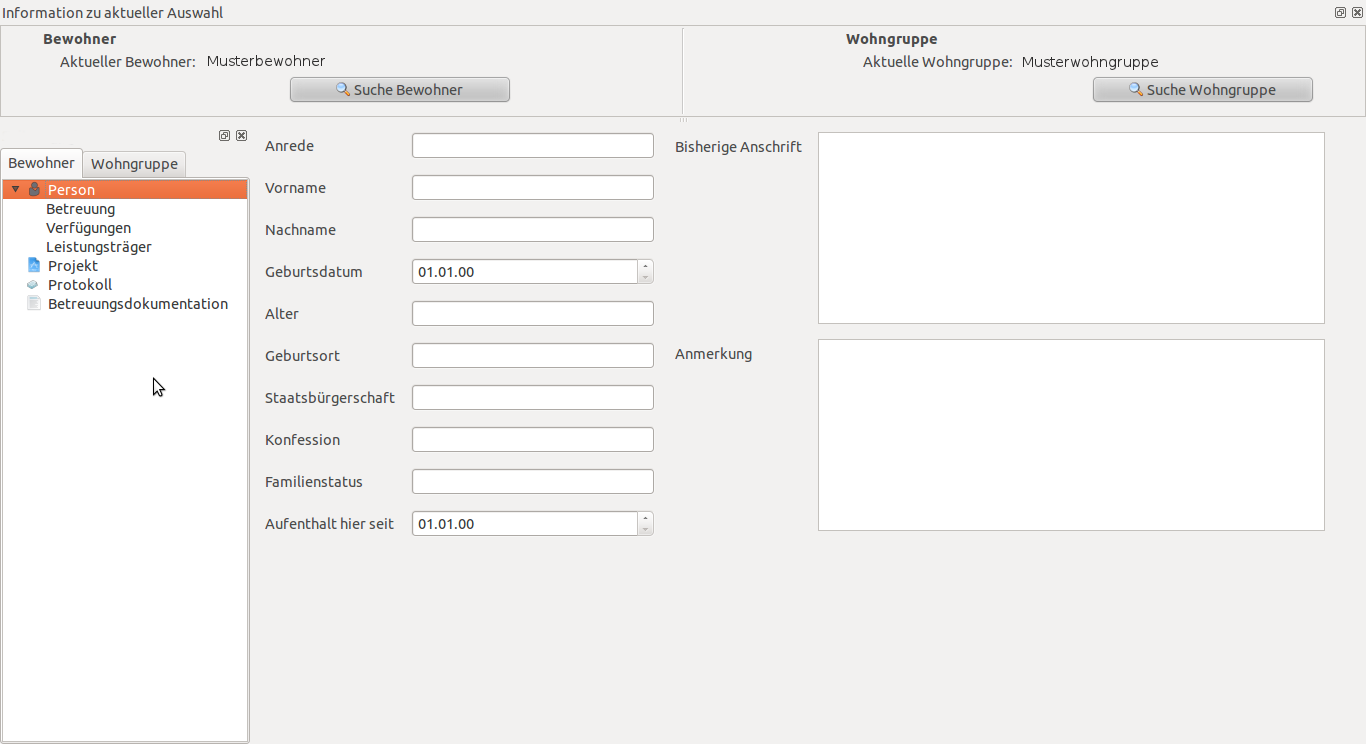
\includegraphics[angle=90, width=\textwidth, height=\textheight]{BewohnerInfo}
\caption{Maske für die personenbezogenen Daten der Bewohner}
\label{Info}
\end{figure}
\begin{figure}
 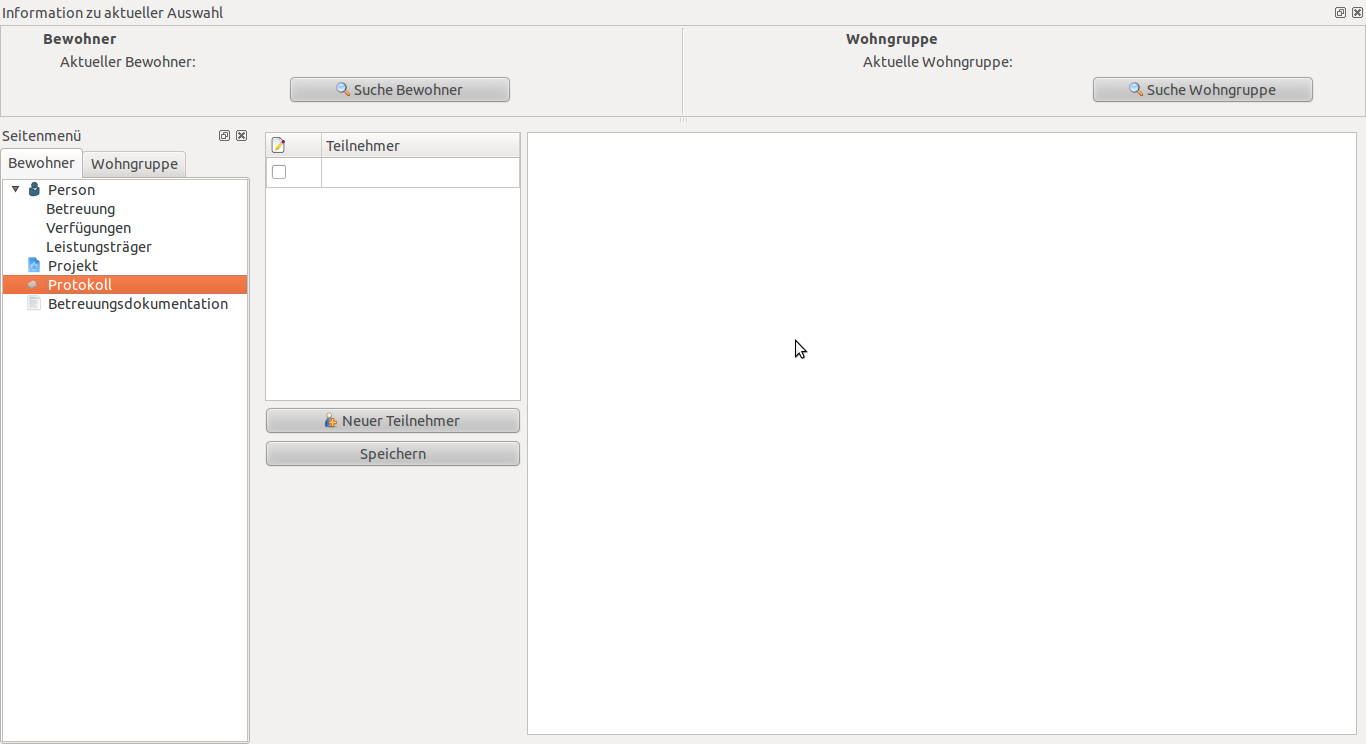
\includegraphics[angle=90, width=\textwidth, height=\textheight]{BewohnerProtokoll}
\caption{Maske für die Protokollfunktion}
\label{Protokoll}
\end{figure}


\end{document}
